\subsection{Attitude Controller Simulation}
The performance of the attitude controller is evaluated by simulating it in the non-linear model. The simulation with the linearized model is not shown due to being almost identical to that of the non-linear model. \autoref{fig:AttitudeController} and \ref{fig:AttitudeControllerOutput} show the performed simulations.
\begin{figure}[H]
	\centering
	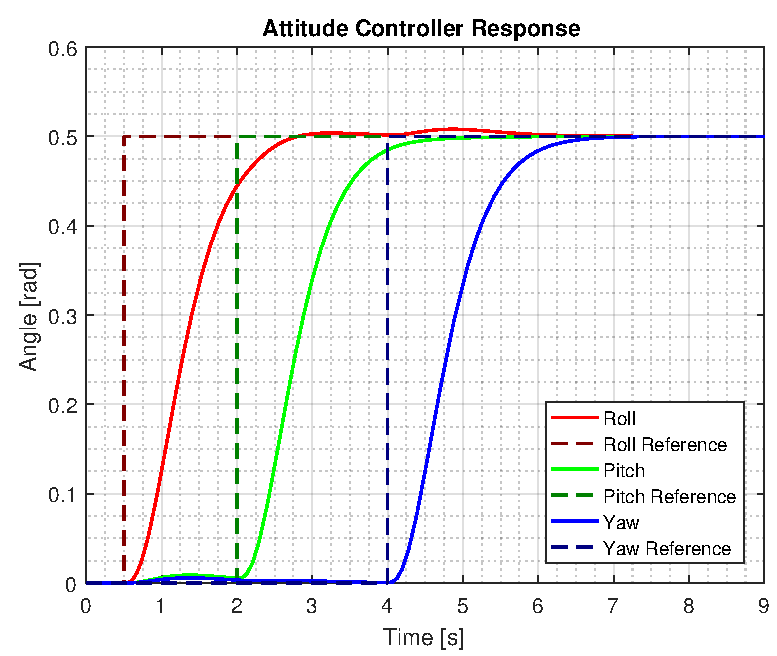
\includegraphics[scale=0.65]{figures/simAttitudeControl}
	\caption{Step response of the attitude controller.}
	\label{fig:AttitudeController}
\end{figure}
It can be seen that the controller reaches the given reference in approximately 2 seconds for the three angles. The coupled charateristic of the system is also present in the graphs as small bumps in two of the angles when the third angle is changed. The controller is capable of handling this situation.

The control action required to achieve the previously seen response is shown in below. 
\begin{figure}[H]
	\centering
	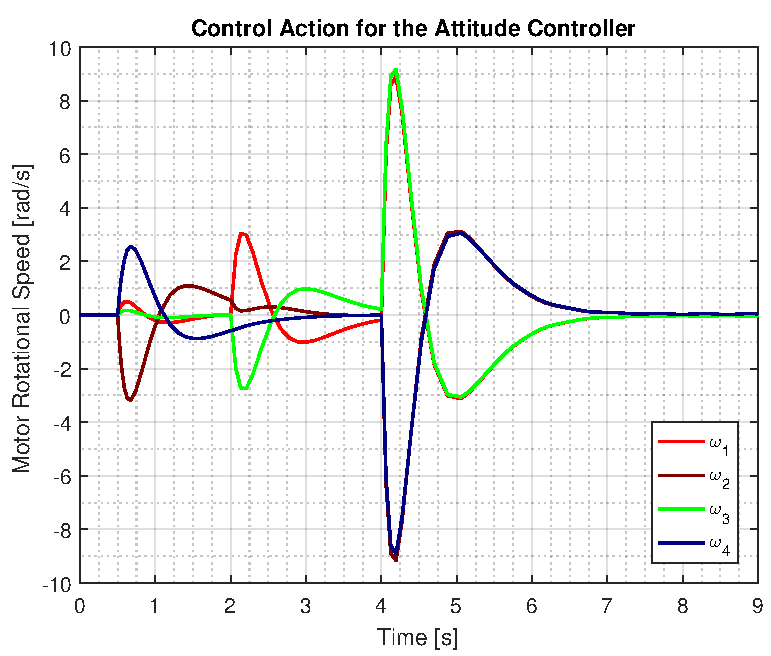
\includegraphics[scale=0.65]{figures/simAttitudeControlOutput}
	\caption{Control output of the attitude controller, that is, the four motor rotational speeds.}
	\label{fig:AttitudeControllerOutput}
\end{figure}
The required motor rotational speeds are represented as variations from the equilibrium rotational speeds of the motors. It can be seen that motors 1 and 3 change their speed when the roll angle is to be changed and motors 2 and 4 do the same for the pitch angle. In these cases, the maximum variation from equilibrium is approximately 3 rad/s. When the yaw angle is to be changed, the four rotational speeds are involved, requiring a peak variation of approximately 9 rad/s. 